%---- Sample WMSU BSMATH BEAMER template ------
%---- Begin editing after PREAMBLE END at line 77------
%---- Created by: Christle Jude L. Maquilan - April 2022 --
%---- @jmaq03.jm@gmail.com -----

\documentclass[xcolor=dvipsnames,envcountsect]{beamer}

%------------------------------------------------
%------------------------------------------------
%------------------------------------------------
%------------------------------------------------
%------------------------------------------------
%----------▼▼▼▼▼ START PREAMBLE ▼▼▼▼▼----------

%-------- theme --------
\usetheme{Madrid}

%-------- color --------
\definecolor{crimsonred}{RGB}{153,0,0} % Official RGB code for Crimson Red
\usecolortheme[named=crimsonred]{structure}
%-------- set color of 'example block' to crimson theme --------
\setbeamercolor{block body example}{bg=white}
\setbeamercolor{block title example}{fg=white, bg=red!50!black}

%-------- font --------
\setbeamerfont{structure}{family=\rmfamily,series=\bfseries}
\usefonttheme[stillsansseriftext]{structurebold}
\setbeamerfont{section in head/foot}{size=\tiny}

%-------- misc structure --------
\useoutertheme[footline=authortitle,subsection=false]{miniframes}
\useinnertheme{rounded}
\addtobeamertemplate{block begin}{}{\justifying}
\newtheorem{remark}[theorem]{Remark}
\renewcommand{\indent}{\hspace*{2em}}
\setbeamertemplate{theorems}[numbered]
\setbeamertemplate{caption}[numbered]
\usepackage[justification=centering]{caption}
\renewcommand{\qedsymbol}{$\blacksquare$}

%-------- packages to be used -------
\usepackage{amsmath,amsfonts,amssymb,amscd,amsthm}
\usepackage{graphicx,xcolor,comment}
\usepackage{mathrsfs} 
\usepackage{multirow}
\usepackage{array}
\usepackage{hyperref}
\usepackage{multicol}
\usepackage{ragged2e}
\usepackage{caption}
\usepackage[french]{babel}
\usepackage{rotating}
\usepackage{enumerate}
\usepackage{tikz}
\usepackage{bm}
\usepackage{csquotes}

%-------- for bibliography -----------------
\usepackage{biblatex}
\setbeamertemplate{bibliography item}{\insertbiblabel}
\addbibresource{References.bib}
\setbeamertemplate{frametitle continuation}{\frametitle{\color{white}List of References}}

%-------- WMSU Backgound -------------------
%\usebackgroundtemplate{%
%	\tikz[overlay,remember picture] \node[opacity=0.02, at=(current page.center)] {
%		
\includegraphics[height=4.5in,width=4.5in]{./Figures/WMSU LOGO.png}};
%}

%----------▲▲▲▲▲ PREAMBLE END ▲▲▲▲▲----------
%------------------------------------------------
%------------------------------------------------
%------------------------------------------------
%------------------------------------------------
%------------------------------------------------

%---------START EDITING HERE---------------------
\title[Études des systèmes GNSS des smartphones]{Études des systèmes GNSS des smartphones}

\author [Noë Charlier]{\textbf{Noë Charlier}}

\institute[Lycée Paul Constans] {\emph{Professeurs: }\textbf{C. Delacour, M. Petitcuenot}\\[1em]
	Classe préparatoire aux grandes écoles\\PT\\Lycée Paul Constans\\[1em]

\includegraphics[scale=0.4]{./Figures/logo Paul Constans.jpg}}

\date[2022 - 2023]{\footnotesize TIPE - \textbf{2022, 2023}}
%--------- START DOCUMENT ------------------
\begin{document}
	
\begin{frame}{\titlepage}\end{frame}
\begin{frame}{\frametitle{Sommaire}\tableofcontents}\end{frame}
%--------- Sujet et Domaine ----------------------
\section{Introduction}
\begin{frame}
	\frametitle{Introduction}
		\justifying
		\textit{Besoin grandissant de solution GNSS:}
		\begin{center}
			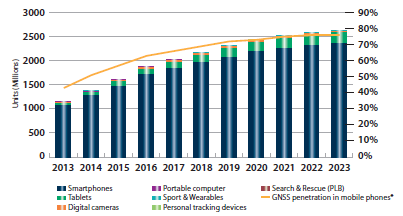
\includegraphics[scale=0.8]{./Figures/stats.png} \\
			{\footnotesize Appareils GNSS par plate-forme. \textit{Market report, ESA}}
		\end{center}
\end{frame}
\begin{frame}
	\frametitle{Définition GNSS}
		\justifying
		\textbf{GNSS:} \textit{Global Navigation Satellite System} (Système de navigation par satellite global)\\
		Constellation de satellites permettant de localiser un point sur la Terre.
\end{frame}
%---------- DEFINITION/PRELIMINARY ---------------------
\section{Motivations}
\begin{frame}
	\frametitle{Motivations du TIPE}
	    \justifying
	    \textbf{Motivations:} 
	    \begin{itemize}
            \item \textbf{Précision du GNSS} - Demande d'une précision du GPS en Ville.
            \item \textbf{Etude physique de l'atomsphère} - Quel impact à l'atmosphere.
            \item \textbf{Informatiques} - Utilisation d'outils de modélisations.
        \end{itemize}
\end{frame} 

%----------- MAIN RESULTS ------------------------------
\section{Objectifs \& Expérimentations}
\begin{frame}{Expérimentations (\& Simulations numérique) et Objectifs}
        \textbf{Expérimentations:} 
	    \begin{itemize}
            \item \textbf{Etude du lien entre SID et précision GPS} - Capteur GPS, et récepteur basse fréquence
        \end{itemize}
        \textbf{Modélisations:} 
	    \begin{itemize}
            \item \textbf{Système GPS réduit} - Modélisation d'un système de résolution GPS afin de lien les résultats expérimentaux.
        \end{itemize}
	%\indent To see this, consider graphs $G_{1}=P_{3}, G_{2}=P_{4}$, and $G_{3}=C_{8}$ in Figure \ref{3.1}.
\end{frame}
\section{Positionnement thématique}
\begin{frame}
	\frametitle{Positionnement thématique}
		\justifying
		%\newline
		%\newline
		\textbf{Positionnement thématique:}
		\begin{itemize}
            \item \textbf{Physique} - Physique Interdisciplinaire
            \item \textbf{Sciences Industrielles} - Traitement du Signal \& Électronique
            \item \textbf{Informatiques} - Informatique Pratique
            \item \textbf{Mathématiques} - Mathématiques Appliquées
        \end{itemize}
\end{frame}
%--------- THANK YOU Text ------- texlive-most -------------------
\begin{frame}
		\centering
		\begin{block}
			\scshape
				\begin{center}
					\Huge\emph{Des Questions ?}
				\end{center}
		\end{block}
\end{frame}
%----------------------------------------------------
\end{document}
